\section{Potential of time-varying adaptation}
\label{sec:potential}

The basic premise of \name is that videos and the characteristics of video analytics pipelines exhibit substantial dynamics over time. As a result, to achieve the "best" resource-accuracy tradeoff, we need to continuously adapt the configurations of the video pipelines. In this section, we demonstrate the value of continuous adaptation by comparing two simple policies 
% In this section, we show that the performance of video analytics, in terms
% of accuracy and resource consumption, could be significantly improved by 
% if we periodically update \nn configurations at a fine-grained timescale.
%At the same time, however, realizing this potential in practice 
%introduces a great cost in resource consumption, which will be addressed
%in the next section.
%To show the potential benefits of dynamically switching configurations,
%To show such dynamics in our settings, we compare two basic policies 
for selecting \nn configurations.

\begin{packedenumerate}
\item {\em One-time update:}
This is an one-time offline policy that exhaustively profiles all configurations on the first $x$ seconds of the 
video, picks the cheapest configuration that has at least $\alpha$ 
accuracy, and sticks with it for the whole duration of the video
(\eg~\cite{videostar}); we use $x=10$.
\item {\em Periodic update:}
This policy divides the video into $T$-second intervals, and profiles all configurations in each interval for the first $t$ seconds of that interval. It then sticks with the cheapest configuration whose accuracy is greater than $\alpha$ for the rest of the interval, \ie for $T-t$ seconds. For our experiments we use $T = 4$, and $t = 1$.
\end{packedenumerate}

%\ga{Are you using pipeline A or B?}

\begin{figure}[t]
    \centering
    \hspace{-0.5cm}
    \subfloat[Pipeline A]
    {
        % 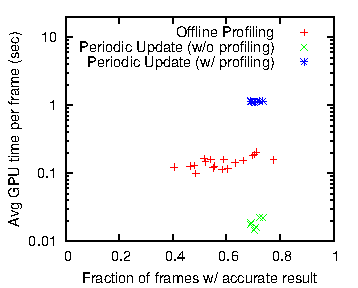
\includegraphics[width=0.25\textwidth]{PaperGraphs/Performance_Upfront_accThresh_70_Optimal.pdf}
        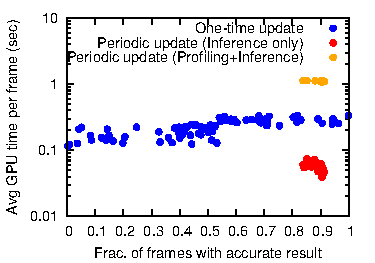
\includegraphics[width=0.25\textwidth]{EvalGraphs/Potential_Improvement.pdf}
        \label{subfig:1}
    }
    \subfloat[Pipeline B]
    {
        % 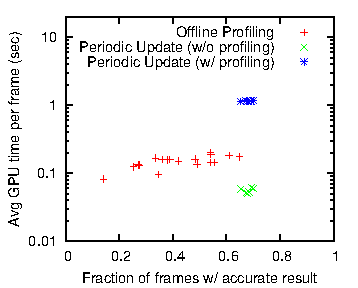
\includegraphics[width=0.25\textwidth]{PaperGraphs/Performance_Upfront_accThresh_80_Optimal.pdf}
        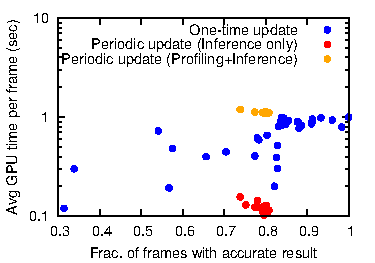
\includegraphics[width=0.25\textwidth]{EvalGraphs_Classifier/Potential_Improvement.pdf}
        \label{subfig:2}
    }
    \caption{Potential improvement of updating the \nn configuration periodically (every $T = 4$ seconds). Ignoring profiling, both accuracy and cost significantly improve (red), but when profiling is factored in, the cost is much worse (yellow) than one-time profiling.}
    \label{fig:potential-impr}
\end{figure}

% \begin{figure}
%     \centering
%     \hspace{-0.5cm}
%     \subfloat[Video clip \#1]
%     {
%         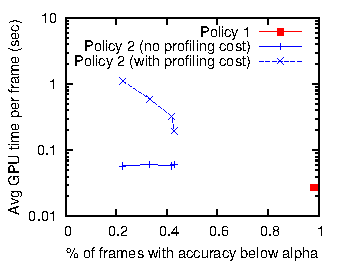
\includegraphics[width=0.25\textwidth]{figures/Bellevue_116th_NE12th_accThresh_80p_Comparison_Policy12.pdf}
%         \label{subfig:1}
%     }
%     \subfloat[Video clip \#2]
%     {
%         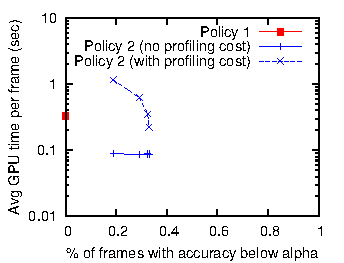
\includegraphics[width=0.25\textwidth]{figures/Bellevue_150th_Eastgate_accThresh_80p_Comparison_Policy12.pdf}
%         \label{subfig:2}
%     }
%     \caption{Performance of one video clip (towards the lower left corner
%     the better).
%     Periodically switching configurations can potentially 
%     reduce resource consumption or raise accuracy relative to offline
%     search  at the cost of increased profiling cost.
%     The solid line shows the resource consumption of the chosen 
%     configuration, and the dash line shows the resource consumption of 
%     both the chosen configuration and the exhaustive search. 
%     Different points represent $T=2,4,8,16$ seconds respectively.}
%     \label{fig:potential}
% \end{figure}

\subsection{Quantifying potential}

%\mypara{Potential improvement}
Figure~\ref{fig:potential-impr} shows the resource-accuracy tradeoffs of running the two
aforementioned policies on 30 traffic videos. 
We set the targeted accuracy threshold $\alpha$ to $0.7$ and $0.8$, respectively. 
(we observe similar results with other thresholds). 
As shown in Figure~\ref{fig:potential-impr}, the periodic policy (red) provides significant improvements over the one-time policy (blue). Indeed, the periodic policy not only reduces per-frame resource consumption by over $10\times$, but also improves the accuracy by up to 2$\times$ over the one-time policy. 

\mypara{Intuition}
The intuition behind these improvements is that the accuracy of a given configuration can depend heavily on the video content. If the video content becomes more challenging (\eg because traffic moves faster, or there is less lighting) this will negatively impact the accuracy. In this case, we would need to move to another configuration that will increase the accuracy, likely at the expense of using more resources. Similarly, if the video content becomes less demanding, we might have the opportunity to move to another configuration that consumes less resources, while still maintaining the desired accuracy. 

%the accuracy
%of each configuration is sensitive to any changes in the video content. This, in turn, creates room for improving accuracy and resource consumption by adapting configurations over time.

To illustrate this intuition, in Figure~\ref{fig:time-variation}, we plot the accuracy over time for two video clips under the two policies. In Figure~\ref{fig:time-variation:a}, initially the cars are moving  slowly, so the one-time policy picks a low frame sampling rate that is  sufficient to achieve the desired accuracy. After a while, however, the cars start moving much faster, and the low sampling rate is no longer sufficient to  correctly detect them. In contrast, the periodic policy is able to maintain high accuracy by increasing the frame sampling rate. Figure~\ref{fig:time-variation:b} shows the converse: cars start out moving very fast, causing both policies to start with a high frame sampling rate. When the cars slow down, the periodic policy reduces the frame sampling rate and saves GPU resources by over $2\times$ compared to the one-time policy. 
Cases like Figure~\ref{fig:time-variation}, where accuracy varies significantly over time are common in real-world camera streams. 

\begin{figure}[t!]
    \centering
    \hspace{-0.5cm}
    \subfloat[]
    {
        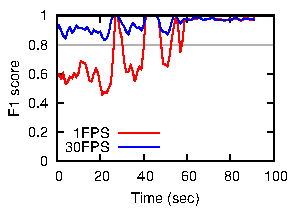
\includegraphics[width=0.25\textwidth]{EvalGraphs/Timeseries_1.pdf}
        \label{fig:time-variation:a}
    }
    \subfloat[]
    {
        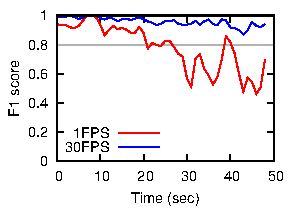
\includegraphics[width=0.25\textwidth]{EvalGraphs/Timeseries_3.pdf}
        \label{fig:time-variation:b}
    }
    \caption{Variation of prediction accuracy over time. The grey line shows the accuracy threshold. If we profile only the first part of the video, we could end up choosing a configuration that is (a) either too resource-demanding, or (b) too inaccurate in the second half of the video.}
    \label{fig:time-variation}
\end{figure}

% \jc{show two concrete examples of accuracy changing over time} \ga{Explain that such changes in videos are common.}

\subsection{Prohibitive profiling cost}
\label{subsec:profiling-cost}

%\mypara{Need for reducing the profiling cost}
While Figure \ref{fig:potential-impr} shows considerable potential for the periodic policy (red), a big caveat is that these results do not include the profiling cost; they only include the cost of running the selected configuration during each time window. Not surprisingly, profiling all configurations every $T$ seconds induces a significant {\em profiling cost}. Worse yet, this profiling cost grows exponentially in the number of configuration knobs and the number of values per knob.

%the average cost of periodic profiling resource consumption per frame (green) {\em did not} include the profiling cost but only the cost of running the chosen configuration. Periodic exhaustive search naturally induces a considerable {\em profiling cost} -- every $T$ seconds, it needs to re-profile the accuracy of all possible configurations, which grows exponentially with the number of knobs and values of each knob. 
% More importantly, unlike the prior work which deals with the profiling 
% cost offline, we require at least some configurations be profiled 
% periodically in real time. 
If done naively, the profiling cost of the periodic policy can negate any gains made by dynamically adapting the configuration. As shown in Figure~\ref{fig:potential-impr}, the total cost when including profiling (yellow) is almost $20\times$ larger than the actual cost of running the selected configuration (red). As a result, the total per-frame cost is even worse than the one-time policy.
%just doing the one-time search for the desired configuration.

%In Figure~\ref{fig:potential-impr}, though periodically updating the configuration every $T$ seconds does find good resource-accuracy 
%trade-offs (green), the profiling cost is almost 20x of actual cost of running the configuration we pick. As a result, the normalized cost per frame including the profiling cost (blue) is worse than just doing the one-time search for the desired configuration.

A sizable component of this profiling cost comes from running the golden configuration. Recall from \S\ref{subsec:profile} that we use the golden configuration as the ground truth for evaluating the accuracy of a given configuration.
%measure the accuracy of the configurations against the golden configuration. 
%\ga{Quantify.} 
On average, running golden configuration requires one-order of magnitude more GPU resource than other configurations. 

\subsection{Challenges in reducing profiling cost}
%\mypara{Why cutting the profiling cost is challenging}
% \jc{explain the balance between selecting a cheaper config and the
% profiling cost to find it}
At the first sight, it might appear that using a state-of-the-art search algorithm (e.g.,~\cite{cherrypick,amazon-bandit}) could address the prohibitively high profiling cost of the periodic policy. Unfortunately, it turns out that these algorithms are inadequate for our particular problem.

%profiling cost could be solved by using a smart search algorithm for a large decision space \cite{examples, of, prior work}, but our setting bears some unique  difficulties that render existing solutions inefficient. 
%First, the accuracy (feedback) of applying an \nn configuration to a live video feed is not instantly revealed; instead, some manually  labeling or, as in our setting, running of a more expensive  configuration on the same video is needed to get the ground truth.

First, existing algorithms are designed for offline settings (\eg find the optimal cloud configuration for a Hadoop application~\cite{cherrypick}). In contrast, our setting is more challenging because we require {\em periodic} profiling, where the cost of a profiling event must be significantly lower than the actual cost of running the selected configuration between two profiling events. 
%updates rather than the whole job; 
%otherwise, the benefit of adaptation would be overwhelmed by profiling
%cost.  
Second, as mentioned above, we need to include the cost of running the golden configuration as part of the profiling cost, which itself can be prohibitively expensive.
%we need the golden configuration to compare and obtain the accuracy of every other configuration. This can be prohibitively expensive. 

Note that simply increasing the update interval $T$ does not help in practice. If the update interval is too large, we might either miss changes in the video content, which could negatively impact  accuracy, or miss opportunities to reduce the resource consumption. 
%the update interval needed becomes too long to capture any dynamics in the accuracies of the configurations.
%reduce the profiling cost, but to make the profiling cost less than actually running the picked configuration, the update interval would be too long to capture any dynamics in accuracy.


% \subsection{\name overview}

% In the next sections, we will present a suite of heuristics to cut the
% re-profiling cost so that we realize the full potential improvement of 
% configuration adaptation.

% We start with the high-level workflow of \name 
% (as outlined in Figure~\ref{}).
% To achieve a desirable resource-accuracy trade-off with minimal
% re-profiling cost, \name uses two techniques: online profiling and 
% cross-video inference. 
% Online profiling (\S\ref{sec:online}) 
% reduces overhead of profiling the performance of a 
% multi-dimensional configuration space by updating different knobs
% separately. 
% In the meantime, cross-video inference (\S\ref{sec:online}) 
% identifies groups of video feeds
% who share similar sweet-spot configurations, so that the online 
% profiling needs to be applied only once to one of the videos.
% A common theme underlying online profiling and cross-video inference
% is the need to generalize profiles spatially and temporally. 
% In \S\ref{sec:transfer}, we introduce a simple technique to 
% how performance profiles learned on one video feed (or 
% time window) can be used to quickly identify the best configuration
% in a different video feed (or time window).
